\section{CLIM Adjust Color limits of plot}

\subsection{Usage}

There are several ways to use \verb|clim| to adjust the color limits of
a plot.  The various syntaxes are
\begin{verbatim}
   clim
   clim([lo,hi])   
   clim('auto')
   clim('manual')
   clim('mode')
   clim(handle,...)
\end{verbatim}
The first form (without arguments), returns a 2-vector containing the
current limits.  The second form sets the limits on the plot to \verb|[lo,hi]|.
The third and fourth form set the mode for the limit to \verb|auto| and \verb|manual|
respectively.  In \verb|auto| mode, FreeMat chooses the range for the axis 
automatically.  The \verb|clim('mode')| form returns the current mode for the axis
(either \verb|'auto'| or \verb|'manual'|).  

Switching to \verb|manual| mode does not change the limits, it simply allows
 you to modify them (and disables the automatic adjustment of the limits
as more objects are added to the plot).  Also, if you specify a set of 
limits explicitly, the mode is set to \verb|manual|
 
Finally, you can specify the handle of an
axis to manipulate instead of using the current one.
\subsection{Example}

Here is an example of using \verb|clim| to change the effective window and
level onto an image.  First, the image with default
limits
\begin{verbatim}
--> x = repmat(linspace(-1,1),[100,1]); y = x';
--> z = exp(-x.^2-y.^2);
--> image(z);
--> min(z(:))

ans = 
    0.1353 

--> max(z(:))

ans = 
    0.9998 
\end{verbatim}
which results in


\centerline{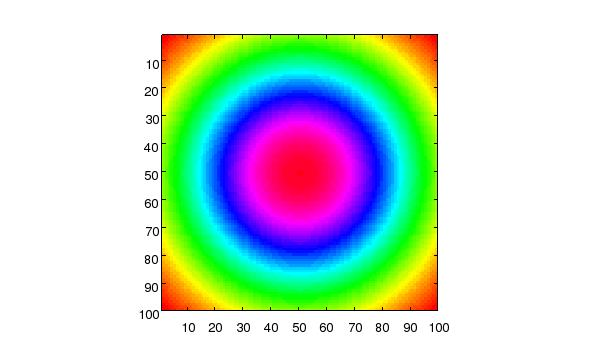
\includegraphics[width=8cm]{clim1}}

Next, we change the colorscale of the image using the
 \verb|clim| function
\begin{verbatim}
--> image(z);
--> clim([0,0.2]);
\end{verbatim}
which results in


\centerline{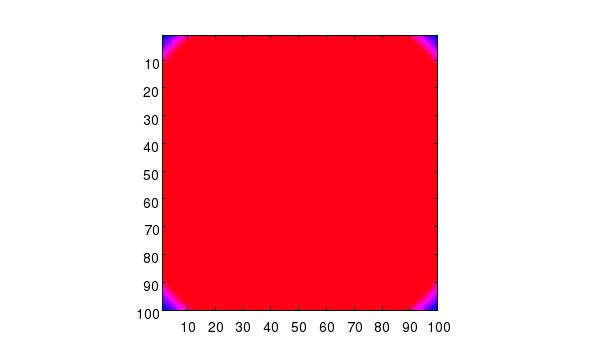
\includegraphics[width=8cm]{clim2}}

